\section{Einführung}
\label{sec:Introduction}


\subsection{Grundideen}
\label{subsec:basic-concepts}
\begin{frame}
	\frametitle{\insertsubsection}
	\begin{itemize}[<+->]
		\item Änderung der Variable hängt von Variable selbst ab

	\end{itemize}
\end{frame}


\subsection{Beispiele}
\label{subsec:examples}
\begin{frame}
    \frametitle{\insertsubsection}
    \begin{itemize}[<+->]
        \item Corona-Neu-Infizierungungen (Änderung) sind proportional zu der Anzahl der bereits infizierten Menschen
        \[\dot{N} = a N\]
        \item[$\Rightarrow$] Exponentielles Wachstum $N=N_0\exp(at)$
        \item Radioaktiver Zerfall: Menge des zerfallenden Materials (Änderung) ist proportional zur Gesamtmenge
        \[\dot{N} = -\lambda N\]
        \item[$\Rightarrow$] Exponentieller Zerfall: $N=N_0\exp(-\lambda t)$
    \end{itemize}
\end{frame}


\subsection{Lösungen für \acsp{ode}}
\label{subsec:solving}
\begin{frame}[fragile]
    \frametitle{\insertsubsection}
    \begin{minted}[linenos, fontsize=\scriptsize, escapeinside=||]{python}
|\pause|import numpy as np
import matplotlib.pyplot as plt

|\pause|def RHS(y, t):
    return -0.5*y

|\pause|if __name__ == "__main__":
    t0 = 0.0
    tend = 10.0
    dt = 1.0
    y0 = 4.0

|\pause|    t_vals = np.arange(t0, tend, dt)
    y_vals = np.array([y0]*len(t_vals))

|\pause|    # Hier wird das Eulersche Verfahren zum lösen der ODE verwendet
    for i in range(len(y_vals)-1):
        y_vals[i+1] = y_vals[i] + dt * RHS(t_vals[i], y_vals[i])

|\pause|    plt.plot(t_vals, y_vals, label="Lösung der Differentialgleichung", marker="o")
    plt.legend()
    plt.show()
	\end{minted}
\end{frame}


\begin{frame}
    \frametitle{\insertsubsection}
    \begin{figure}
        \centering
        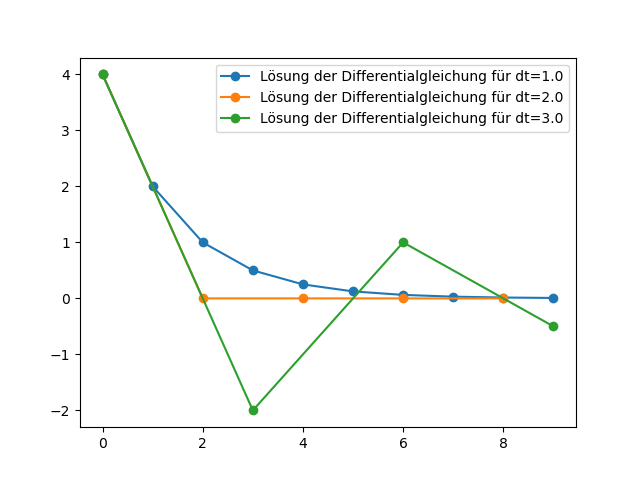
\includegraphics[width=0.7\textwidth]{media/Euler-Solutions_multiple.png}
        \caption{Das Euler-Verfahren löst eine \ac{ode} schrittweise mit konstanter Schrittweite.}
    \end{figure}
\end{frame}


\section{Aufgaben}
\subsection{Aufgabe 1}
\label{subsec:exercise-1}
\begin{frame}
    \frametitle{\insertsubsection}
    \begin{itemize}[<+->]
        \item
    \end{itemize}
\end{frame}


\subsection{Aufgabe 2}
\label{subsec:exercise-1}
\begin{frame}
    \frametitle{\insertsubsection}
    Gegeben ist die folgende Differentialgleichung
    \[\dot{A} = \alpha - \beta A\]
    \begin{enumerate}[<+->]
        \item Löse diese Differentialgleichung numerisch mit dem Euler-Verfahren.\\
        \item Welche Eigenschaften haben die parameter $\alpha,\beta$?
        \item Welche Probleme können auftreten für verschiedene parameter $\alpha,\beta$?
        \item Welches biologische System könnte dieser Differentialgleichung zugrunde liegen?
    \end{enumerate}

\end{frame}


\subsection{Aufgabe 3}
\label{subsec:exercise-1}
\begin{frame}
    \frametitle{\insertsubsection}
    \begin{itemize}[<+->]
        \item
    \end{itemize}
\end{frame}



